\newpage
\section{模型建立与求解}

\subsection{模型一：太空电梯运力与时间线分析}

\subsubsection{问题构建与建模思路}

太空电梯系统代表了地球到轨道运输的范式转变，通过电力驱动实现连续载荷运送，无需燃烧推进。本模型的目标是建立系统的有效吞吐运力并预测仅使用该运输方式完成月球殖民地建设的时间线。

太空电梯的根本优势在于其运营可持续性：系统建成后，通过沿石墨烯系绳的电磁推进移动载荷，将电能直接转换为引力势能。这消除了限制化学火箭的质量比约束，实现了显著更低的单位运输成本。

\subsubsection{系统架构与运力模型}

太空电梯系统由$n = 3$座银河港组成，沿地球赤道间隔120度布置。每座银河港包含：
\begin{enumerate}
    \item 一个地球港口，提供地面基础设施和载荷集结
    \item 两条10万公里石墨烯系绳，延伸至地球同步轨道（GEO，35,786公里）之外
    \item 两个顶点锚点，作为配重和月球运输火箭的中转站
\end{enumerate}

单港理论年运力为$C_e = 179,000$公吨。系统总理论运力为：
\begin{equation}
    C_{e,\text{theoretical}} = n \cdot C_e = 3 \times 179,000 = 537,000 \text{ 公吨/年}
    \label{eq:elevator_theoretical}
\end{equation}

\subsubsection{运营约束与有效运力}

实际运营通过两种主要机制导致运力折减：

\textbf{系统停机}：维护需求、部件故障和紧急维修降低运营可用性。模型采用年故障率$\epsilon_e = 0.02$（2\%），表示系统非运营时间比例。

\textbf{系绳动力学}：尽管问题陈述假设"无摆动"，我们纳入保守的系绳动力学因子$\delta = 0.05$（5\%），以考虑可能降低有效载荷吞吐量的微振动、热膨胀效应和轨道扰动。

有效年运力为：
\begin{equation}
    C_{e,\text{eff}} = C_{e,\text{theoretical}} \cdot (1 - \epsilon_e) \cdot (1 - \delta) = 537,000 \times 0.98 \times 0.95 = \textbf{499,947 公吨/年}
    \label{eq:elevator_effective}
\end{equation}

\begin{figure}[htbp]
    \centering
    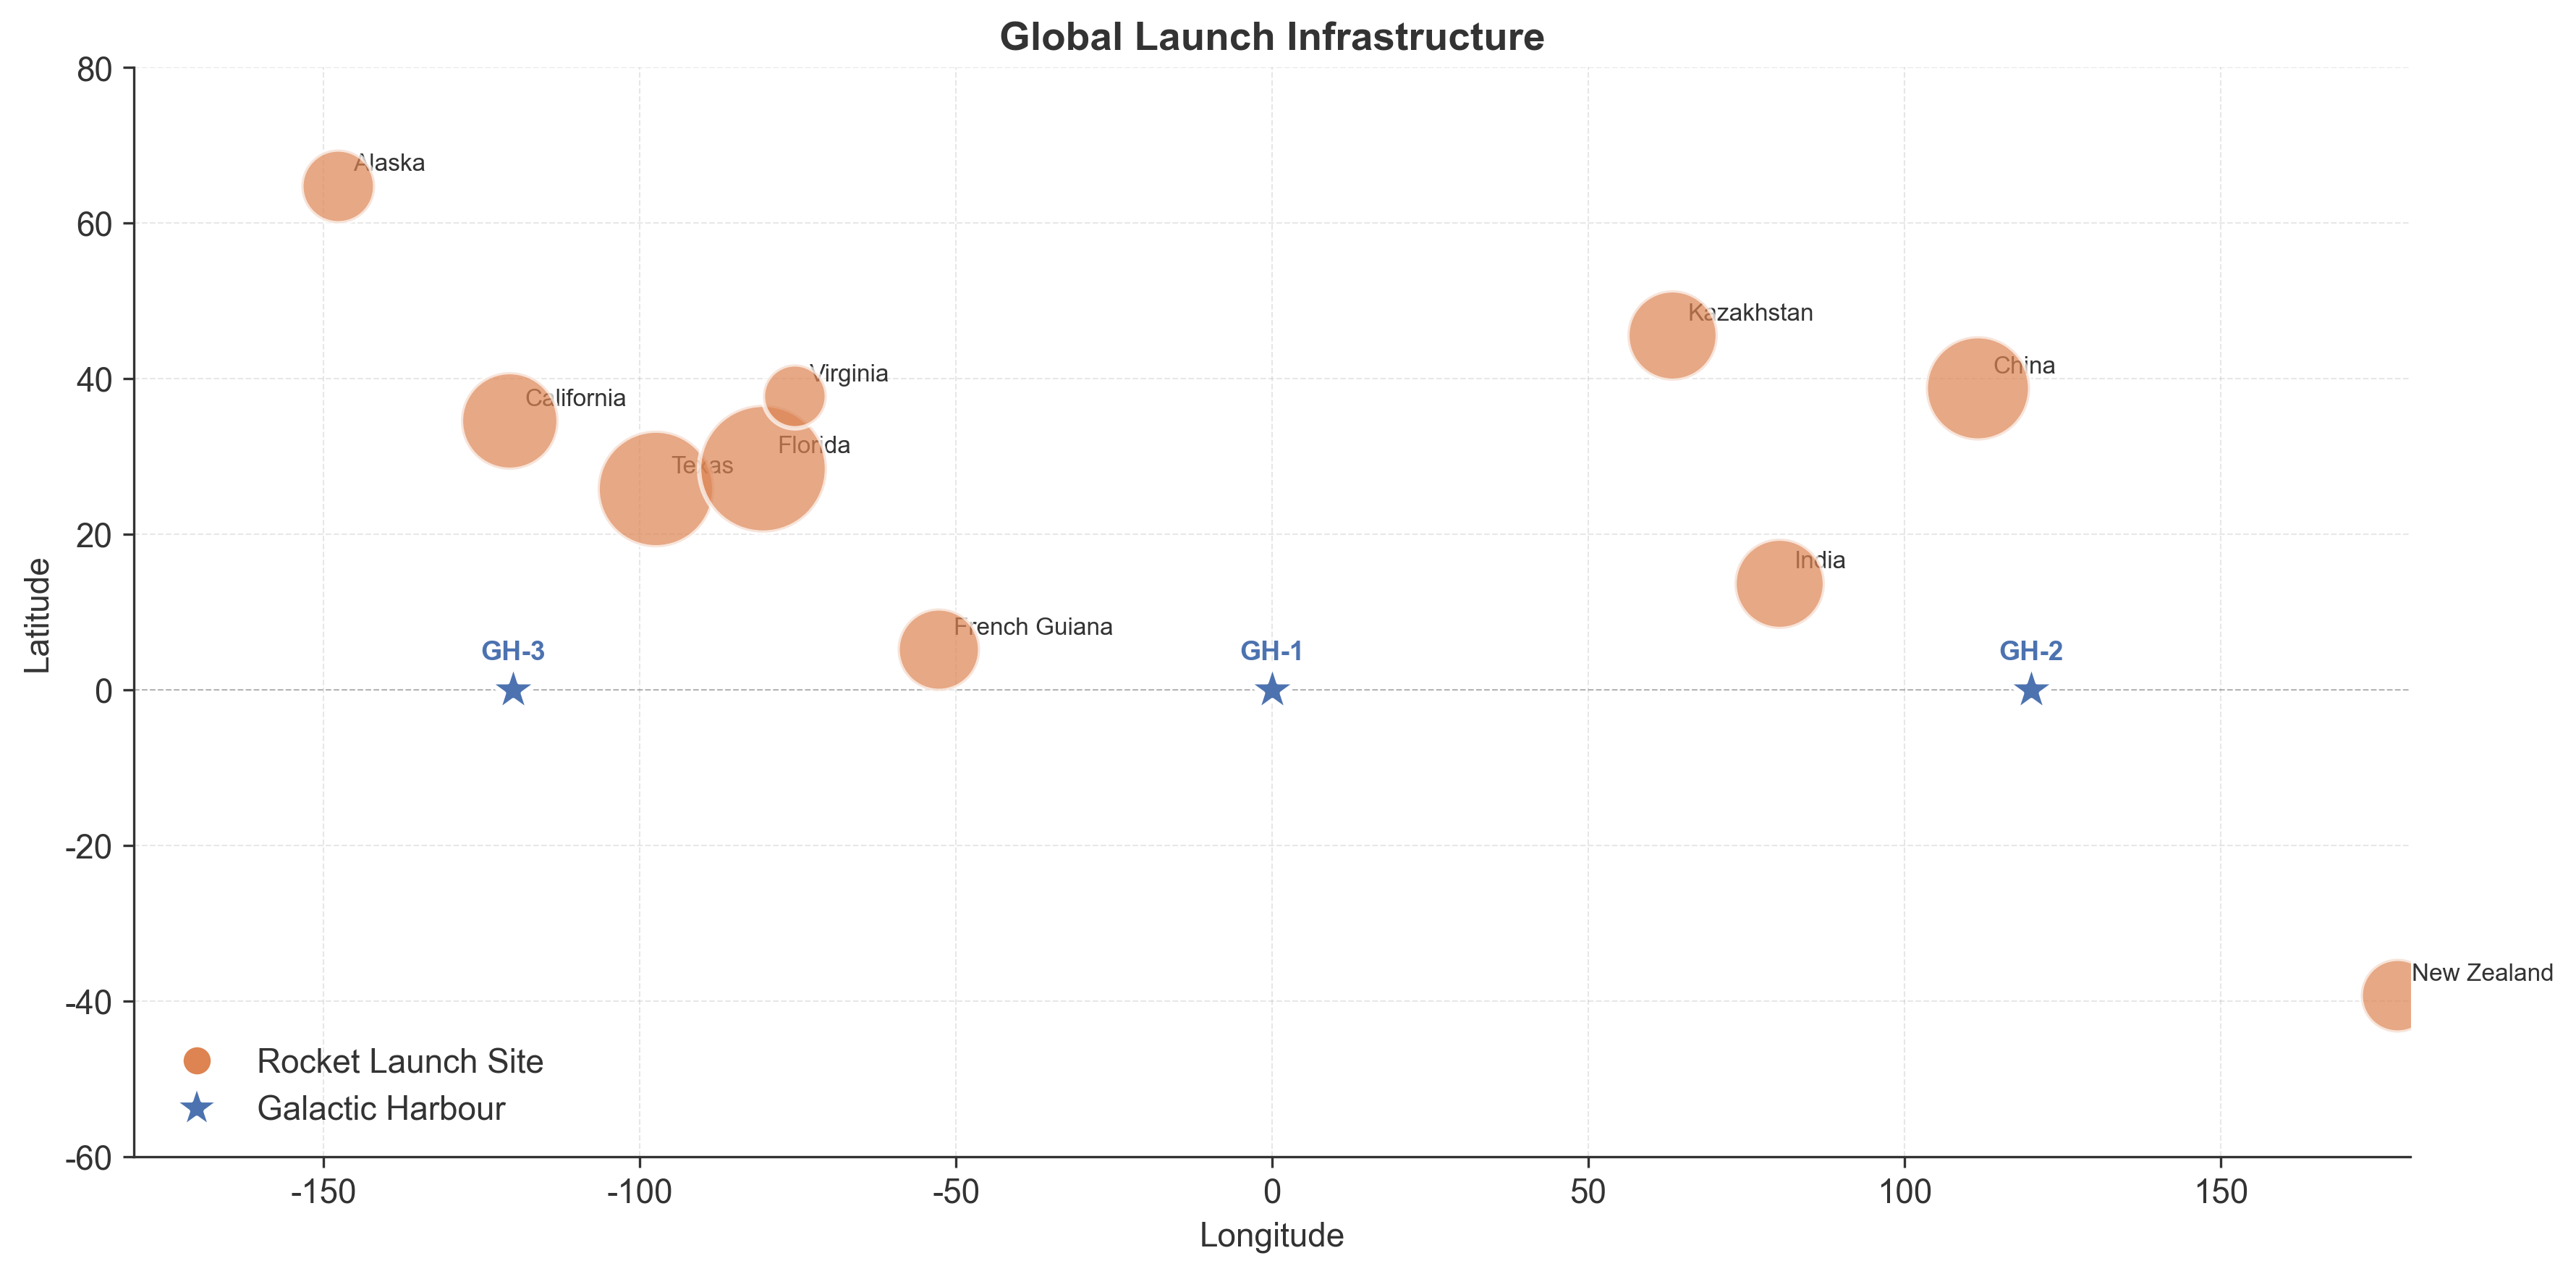
\includegraphics[width=0.85\textwidth]{../figures/fig_06_launch_sites.png}
    \caption{全球运输基础设施分布。蓝色星号表示赤道上的三座银河港位置（GH-1、GH-2、GH-3），橙色圆圈表示火箭发射基地，圆圈大小与年发射能力成正比。}
    \label{fig:launch_sites}
\end{figure}

如图~\ref{fig:launch_sites}所示，银河港最优布置于赤道以最大化地球自转速度优势，而火箭发射基地则基于现有基础设施和地理优势在全球分布。

\subsubsection{时间线与成本预测}

给定总材料需求$M = 100,000,000$公吨，纯电梯方案的建设周期为：
\begin{equation}
    T_{\text{elevator}} = \frac{M}{C_{e,\text{eff}}} = \frac{100,000,000}{499,947} = \textbf{190.0 年}
    \label{eq:elevator_timeline}
\end{equation}

运输成本按电梯成本因子$c_e = 100$美元/公斤计算：
\begin{equation}
    \text{Cost}_{\text{elevator}} = M \times 1000 \times c_e = 100 \times 10^6 \times 1000 \times 100 = \textbf{10 万亿美元}
    \label{eq:elevator_cost}
\end{equation}

环境影响通过CO$_2$排放因子$\gamma_e = 0.1$公吨CO$_2$/公吨载荷（计入发电排放）量化：
\begin{equation}
    E_{\text{elevator}} = M \times \gamma_e = 100 \times 10^6 \times 0.1 = 10 \times 10^6 \text{ 公吨}
    \label{eq:elevator_co2}
\end{equation}

即总排放\textbf{1000万公吨CO$_2$}。

\subsubsection{模型一结果小结}

表~\ref{tab:model1_results}汇总了太空电梯方案的结果。

\begin{table}[htbp]
    \centering
    \caption{纯太空电梯方案结果}
    \label{tab:model1_results}
    \begin{tabular}{lrr}
        \toprule
        指标 & 数值 & 单位 \\
        \midrule
        理论年运力 & 537,000 & 公吨/年 \\
        有效年运力 & 499,947 & 公吨/年 \\
        建设周期 & 190.0 & 年 \\
        完工年份 & 2240 & -- \\
        总成本 & 10.00 & 万亿美元 \\
        单位成本 & 100 & 美元/公斤 \\
        总CO$_2$排放 & 10.00 & 百万公吨 \\
        碳强度 & 0.10 & 公吨CO$_2$/公吨载荷 \\
        \bottomrule
    \end{tabular}
\end{table}

纯电梯方案具有最低成本和环境影响，但需要近两个世纪完成——这一时间跨度挑战了跨代规划的极限。

\subsection{模型二：传统火箭发射网络分析}

\subsubsection{问题构建与网络结构}

传统火箭发射提供了一条具有根本不同特性的替代运输路径：更高的单位成本、地球到月球的直接运送，以及成熟的技术基础。本模型评估10个全球发射设施的总运力并预测任务完成参数。

火箭方案消除了太空电梯的两阶段运输需求（地球港口至顶点锚点，再至月球），改为从地球表面直接向月球目的地运送载荷。这一简化以显著更高的单位能耗为代价。

\subsubsection{发射站点运力模型}

每个发射站点$i$具有年发射能力$\lambda_i$，由基础设施、人员和监管约束决定。基于假设可重复使用火箭技术和发射设施扩张的持续投资，2050年预测的各站点运力如表~\ref{tab:launch_sites}所示。

\begin{table}[htbp]
    \centering
    \caption{全球火箭发射站点规格}
    \label{tab:launch_sites}
    \begin{tabular}{lccc}
        \toprule
        发射站点 & 位置 & 年发射能力（次/年） & 纬度 \\
        \midrule
        美国佛罗里达 & 卡纳维拉尔角 & 600 & 28.5°N \\
        美国德克萨斯 & 博卡奇卡 & 500 & 25.9°N \\
        中国 & 太原 & 400 & 38.8°N \\
        美国加利福尼亚 & 范登堡 & 350 & 34.6°N \\
        哈萨克斯坦 & 拜科努尔 & 300 & 45.6°N \\
        印度 & 萨迪什·达万 & 300 & 13.7°N \\
        法属圭亚那 & 库鲁 & 250 & 5.2°N \\
        美国阿拉斯加 & 科迪亚克 & 200 & 64.8°N \\
        新西兰 & 马希亚 & 200 & 39.3°S \\
        美国弗吉尼亚 & 沃洛普斯 & 150 & 37.8°N \\
        \midrule
        \textbf{合计} & -- & \textbf{3,250} & -- \\
        \bottomrule
    \end{tabular}
\end{table}

理论年载荷运输能力为：
\begin{equation}
    C_{r,\text{theoretical}} = C_r \times \sum_{i=1}^{10} \lambda_i = 125 \times 3,250 = 406,250 \text{ 公吨/年}
    \label{eq:rocket_theoretical}
\end{equation}

其中$C_r = 125$公吨为单次平均载荷（先进猎鹰重型100-150公吨范围的中值）。

\subsubsection{失败率与有效运力}

火箭发射会因多种机制失败：推进异常、制导错误、分离故障和载荷部署问题。成熟火箭系统的历史失败率为2-5\%；我们采用$\epsilon_r = 0.03$（3\%）作为2050年预测值，反映可靠性的持续提升。

有效年运力为：
\begin{equation}
    C_{r,\text{eff}} = C_{r,\text{theoretical}} \times (1 - \epsilon_r) = 406,250 \times 0.97 = \textbf{394,063 公吨/年}
    \label{eq:rocket_effective}
\end{equation}

\subsubsection{时间线、成本与环境预测}

纯火箭方案的建设周期为：
\begin{equation}
    T_{\text{rocket}} = \frac{M}{C_{r,\text{eff}}} = \frac{100,000,000}{394,063} = \textbf{253.8 年}
    \label{eq:rocket_timeline}
\end{equation}

运输成本按$c_r = 1,500$美元/公斤计算：
\begin{equation}
    \text{Cost}_{\text{rocket}} = M \times 1000 \times c_r = 100 \times 10^6 \times 1000 \times 1,500 = \textbf{150 万亿美元}
    \label{eq:rocket_cost}
\end{equation}

环境影响主要来自火箭推进剂燃烧。单次发射CO$_2$排放$\gamma_r = 500$公吨：
\begin{equation}
    E_{\text{rocket}} = \gamma_r \times \frac{M}{C_r} = 500 \times \frac{100,000,000}{125} = 400 \times 10^6 \text{ 公吨}
    \label{eq:rocket_co2}
\end{equation}

即总排放\textbf{4亿公吨CO$_2$}。

\begin{figure}[htbp]
    \centering
    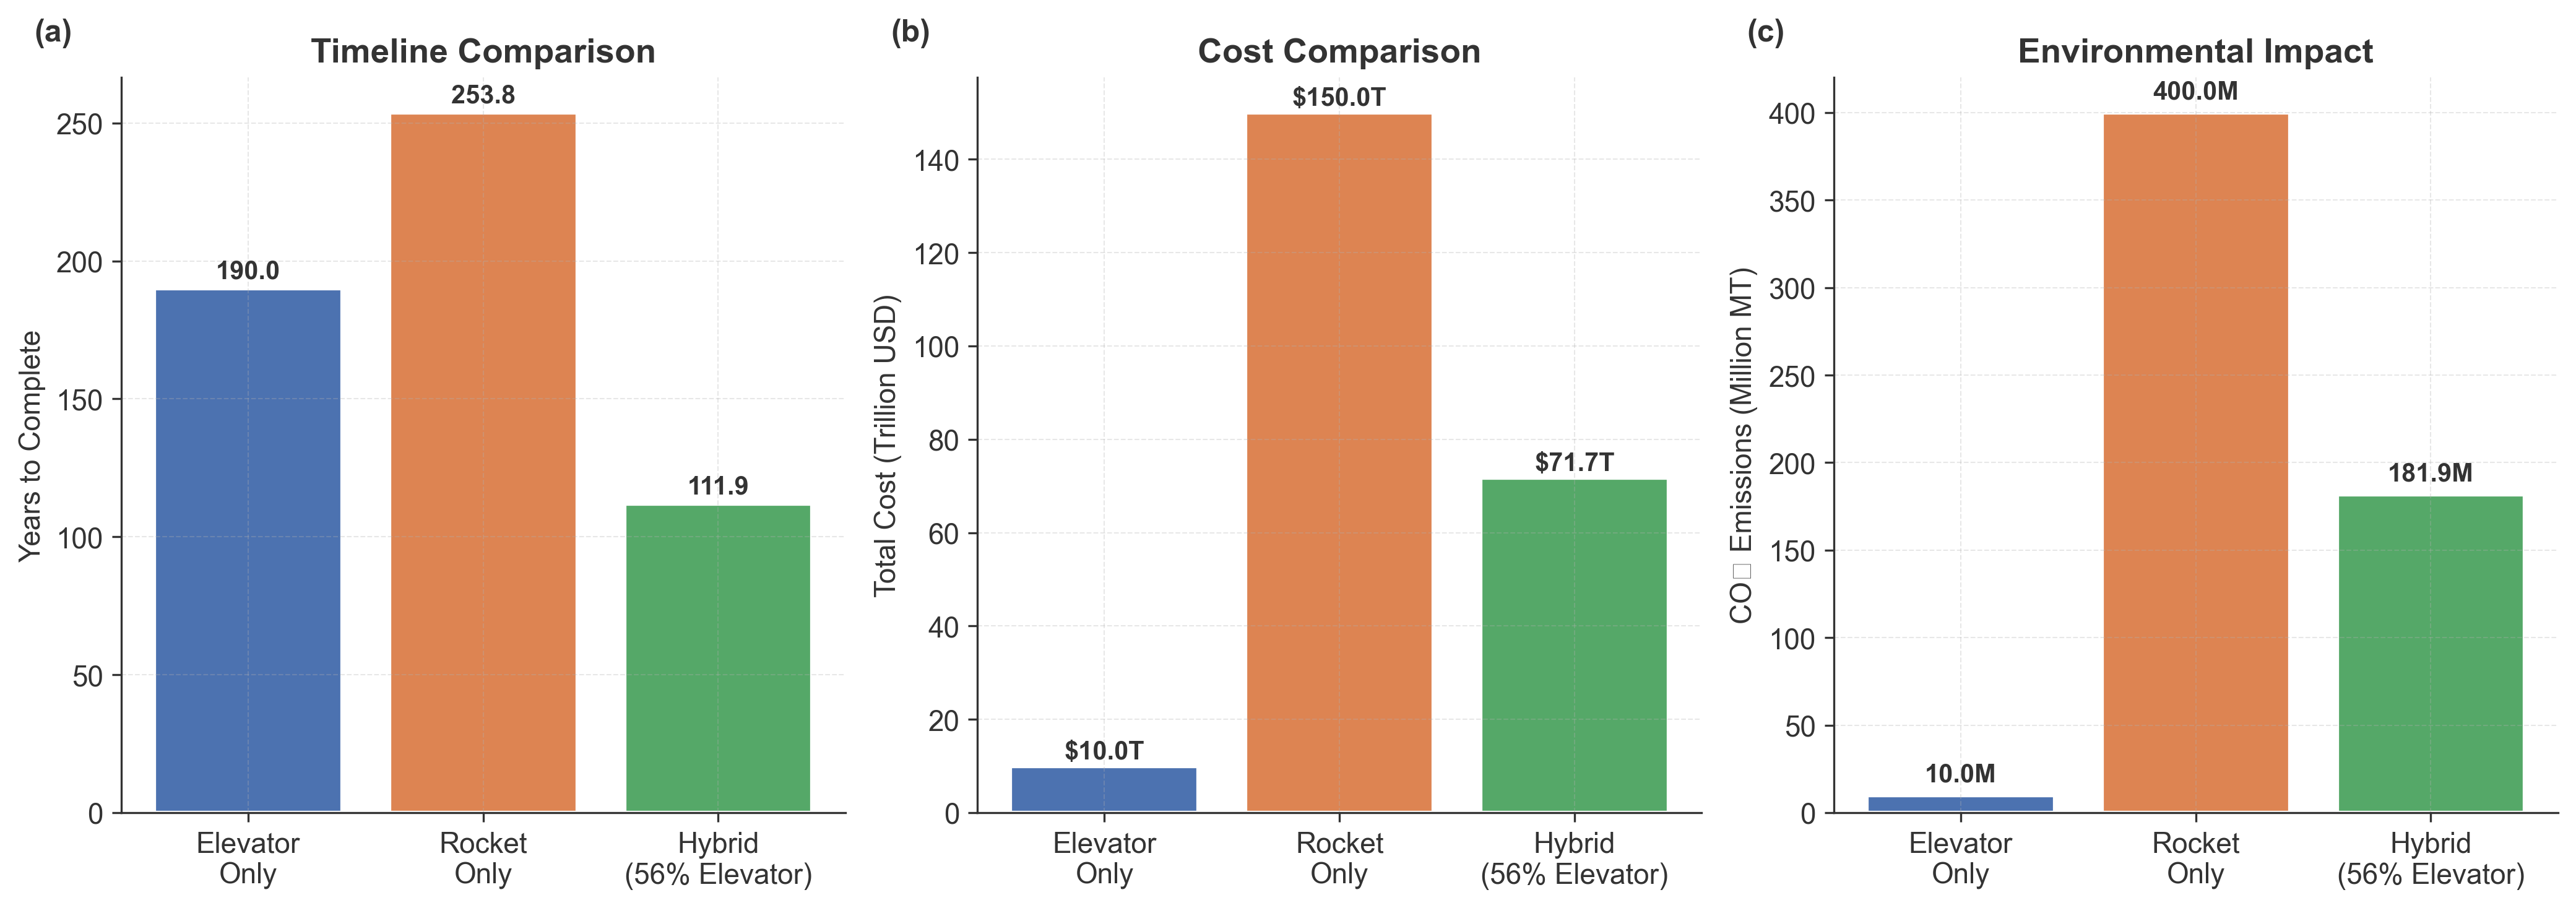
\includegraphics[width=0.95\textwidth]{../figures/fig_01_scenario_comparison.png}
    \caption{三种运输方案比较：(a)建设周期（年），(b)总成本（万亿美元），(c)CO$_2$排放（百万公吨）。混合方案实现了最短工期，同时平衡了成本和环境考量。}
    \label{fig:scenario_comparison}
\end{figure}

如图~\ref{fig:scenario_comparison}所示，纯火箭方案比纯电梯方案需要\textbf{33.6\%}更长时间，成本高\textbf{15倍}，CO$_2$排放高\textbf{40倍}。

\subsubsection{模型二结果小结}

纯火箭方案揭示了纯燃烧基运输用于超大规模太空物流的局限性，其高昂成本和环境影响挑战了任务可行性。

\subsection{模型三：混合运输优化}

\subsubsection{问题构建与优化目标}

混合方案寻求利用两种运输系统的互补优势：太空电梯的低成本和环境效率与火箭的补充运力。核心问题是：\textit{如何在系统间分配材料以最小化总建设时间，同时管理成本和环境约束？}

令$\alpha \in [0,1]$为通过太空电梯运输的材料比例，$(1-\alpha)$为通过火箭运输。优化目标是在运力约束下最小化工期。

\subsubsection{运力比例分配策略}

两系统并行运行时，总有效运力为：
\begin{equation}
    C_{\text{total}} = C_{e,\text{eff}} + C_{r,\text{eff}} = 499,947 + 394,063 = \textbf{894,010 公吨/年}
    \label{eq:total_capacity}
\end{equation}

为最小化工期，材料应按使两系统同时完成交付的方式分配。当满足以下条件时实现：
\begin{equation}
    \frac{\alpha \cdot M}{C_{e,\text{eff}}} = \frac{(1-\alpha) \cdot M}{C_{r,\text{eff}}}
    \label{eq:simultaneous_completion}
\end{equation}

求解最优分配比例：
\begin{equation}
    \alpha^* = \frac{C_{e,\text{eff}}}{C_{e,\text{eff}} + C_{r,\text{eff}}} = \frac{499,947}{894,010} = \textbf{0.559}（55.9\%）
    \label{eq:optimal_alpha}
\end{equation}

该\textbf{运力比例分配}确保整个建设期间两系统均获得最大利用。

\subsubsection{优化时间线与资源配置}

最优分配下，建设周期为：
\begin{equation}
    T_{\text{hybrid}} = \frac{M}{C_{\text{total}}} = \frac{100,000,000}{894,010} = \textbf{111.9 年}
    \label{eq:hybrid_timeline}
\end{equation}

材料分配：
\begin{align}
    M_{\text{elevator}} &= \alpha^* \times M = 0.559 \times 100,000,000 = \textbf{5592万公吨} \\
    M_{\text{rocket}} &= (1-\alpha^*) \times M = 0.441 \times 100,000,000 = \textbf{4408万公吨}
    \label{eq:material_allocation}
\end{align}

\begin{figure}[htbp]
    \centering
    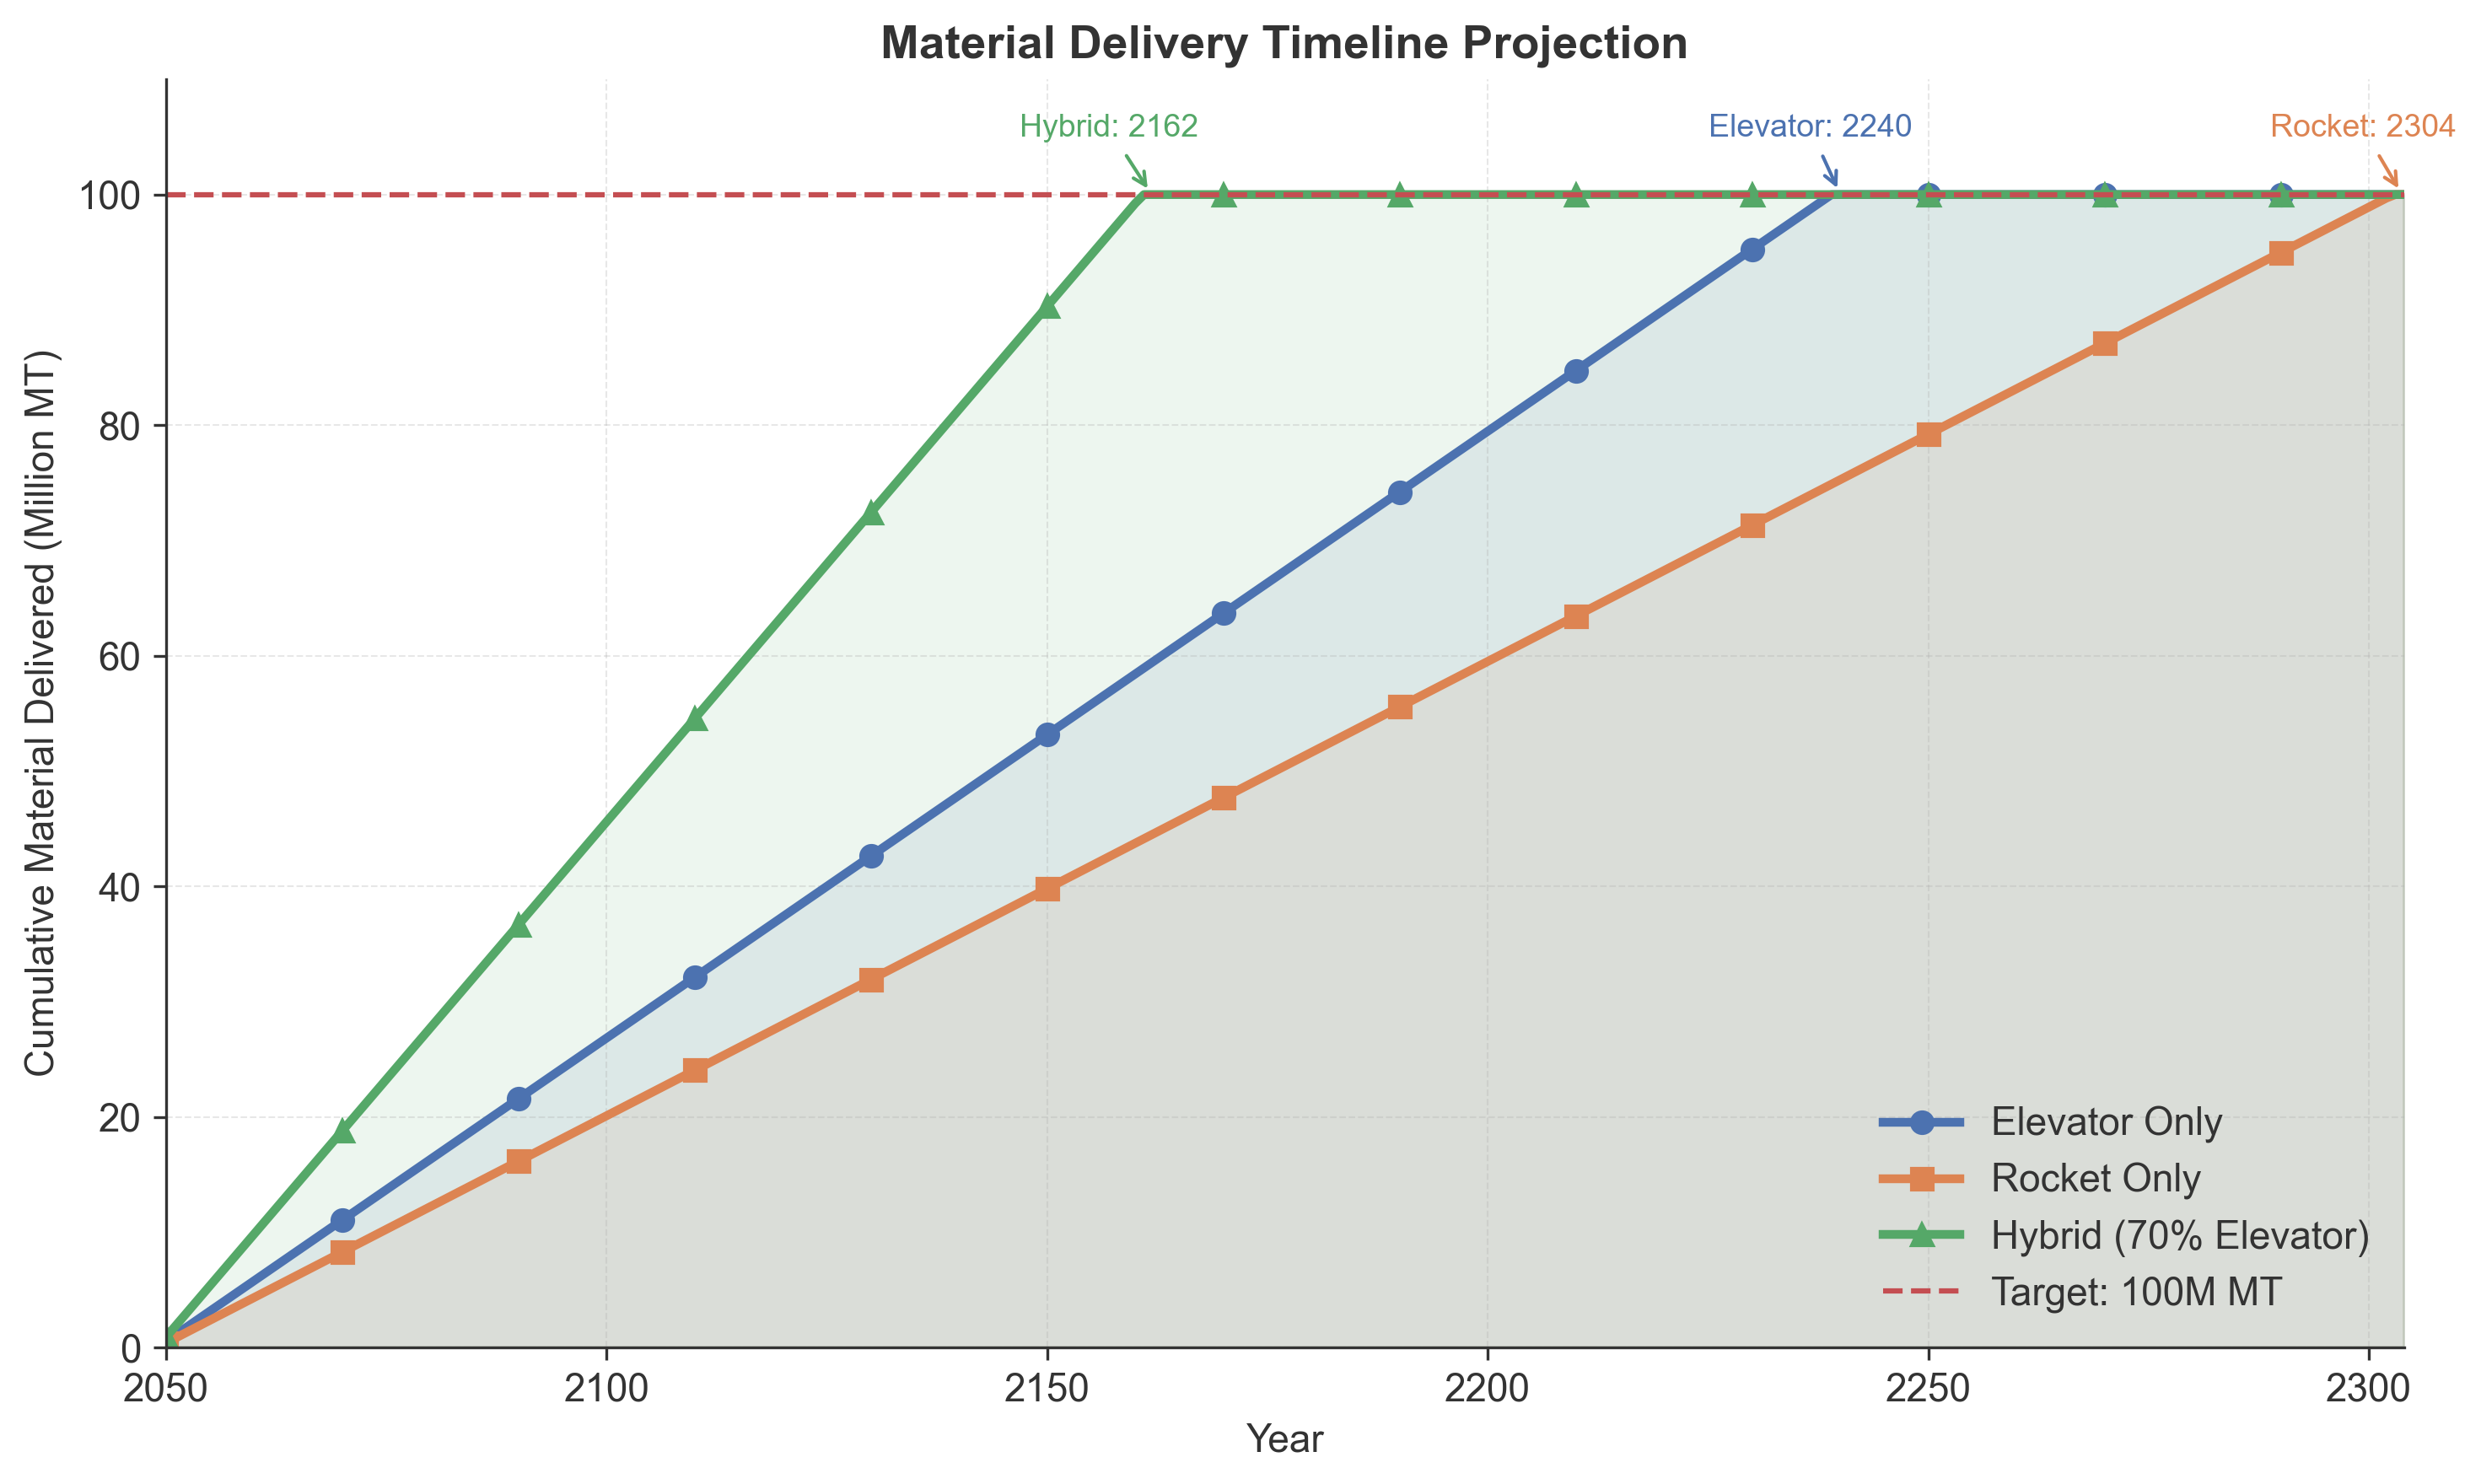
\includegraphics[width=0.95\textwidth]{../figures/fig_03_timeline_projection.png}
    \caption{三种方案的累计材料运送时间线预测。混合方案（绿色）显著快于任一单模式方案达到1亿公吨目标，预计于2162年完工。}
    \label{fig:timeline_projection}
\end{figure}

图~\ref{fig:timeline_projection}可视化了累计运送轨迹，展示了并行运营如何显著加速任务完成。

\subsubsection{成本与环境分析}

混合配置下的总成本：
\begin{align}
    \text{Cost}_{\text{hybrid}} &= M_{\text{elevator}} \times 1000 \times c_e + M_{\text{rocket}} \times 1000 \times c_r \nonumber \\
    &= 55.92 \times 10^6 \times 1000 \times 100 + 44.08 \times 10^6 \times 1000 \times 1,500 \nonumber \\
    &= 5.59 + 66.12 = \textbf{71.71 万亿美元}
    \label{eq:hybrid_cost}
\end{align}

环境影响：
\begin{align}
    E_{\text{hybrid}} &= M_{\text{elevator}} \times \gamma_e + \frac{M_{\text{rocket}}}{C_r} \times \gamma_r \nonumber \\
    &= 55.92 \times 10^6 \times 0.1 + \frac{44.08 \times 10^6}{125} \times 500 \nonumber \\
    &= 5.59 + 176.31 = 181.9 \times 10^6 \text{ 公吨}
    \label{eq:hybrid_co2}
\end{align}

即总排放\textbf{1.819亿公吨CO$_2$}。

\begin{figure}[htbp]
    \centering
    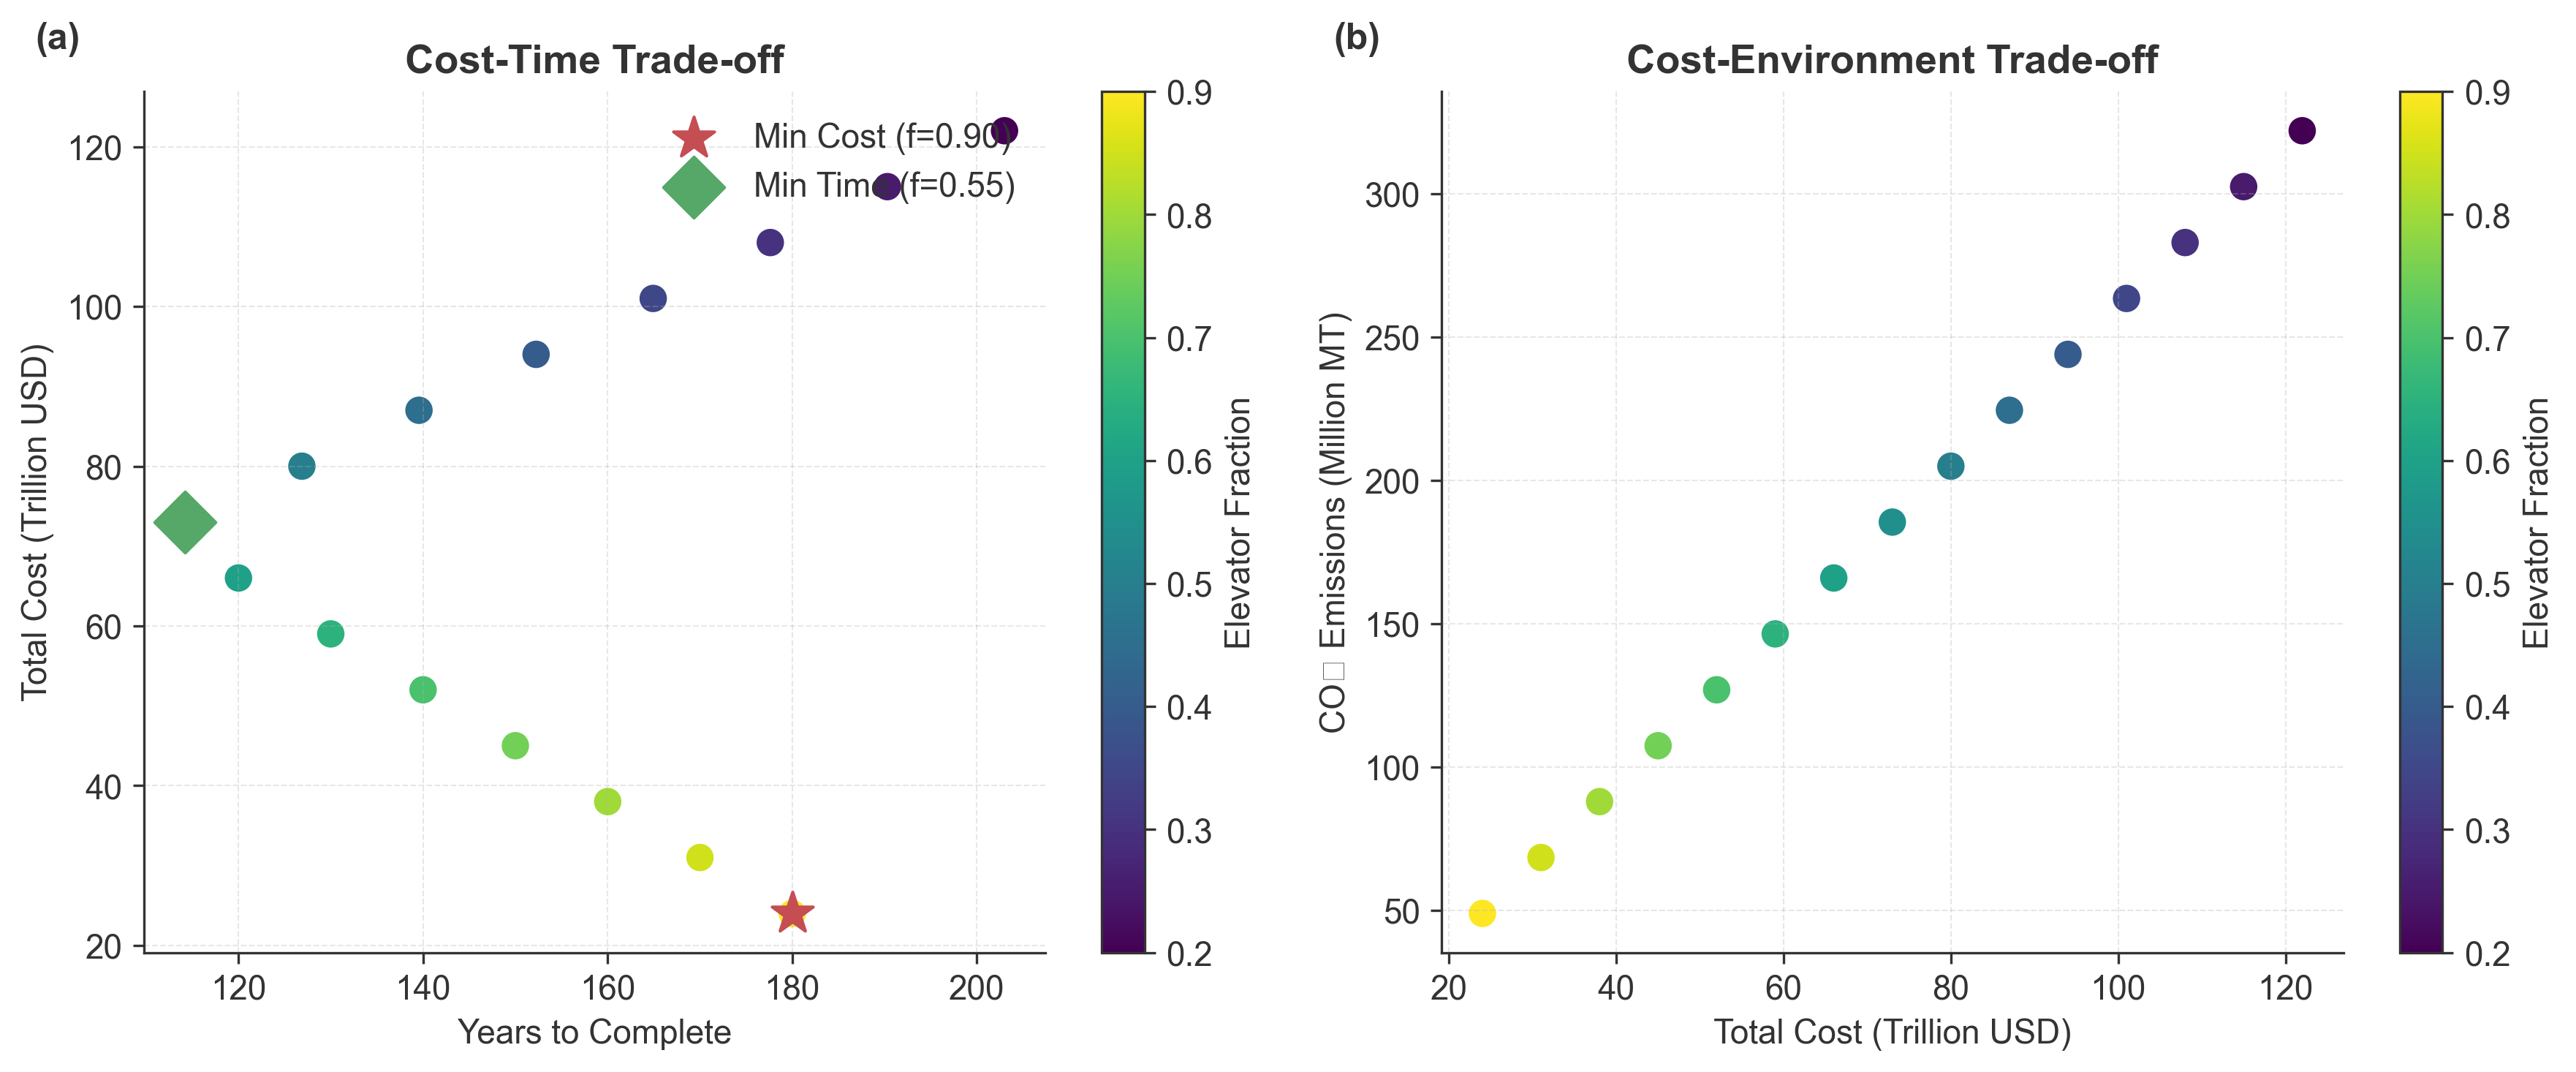
\includegraphics[width=0.95\textwidth]{../figures/fig_02_optimization_tradeoff.png}
    \caption{混合配置权衡分析：(a)成本与工期关系，展示帕累托前沿，颜色表示电梯比例；(b)成本与CO$_2$排放权衡。红色星号标记最低成本配置；绿色菱形标记最短工期（最优运力比例分配）。}
    \label{fig:optimization_tradeoff}
\end{figure}

图~\ref{fig:optimization_tradeoff}展示了不同分配策略的权衡空间。运力比例分配（绿色菱形）实现最短工期，而其他分配可以降低成本但延长工期。

\begin{figure}[htbp]
    \centering
    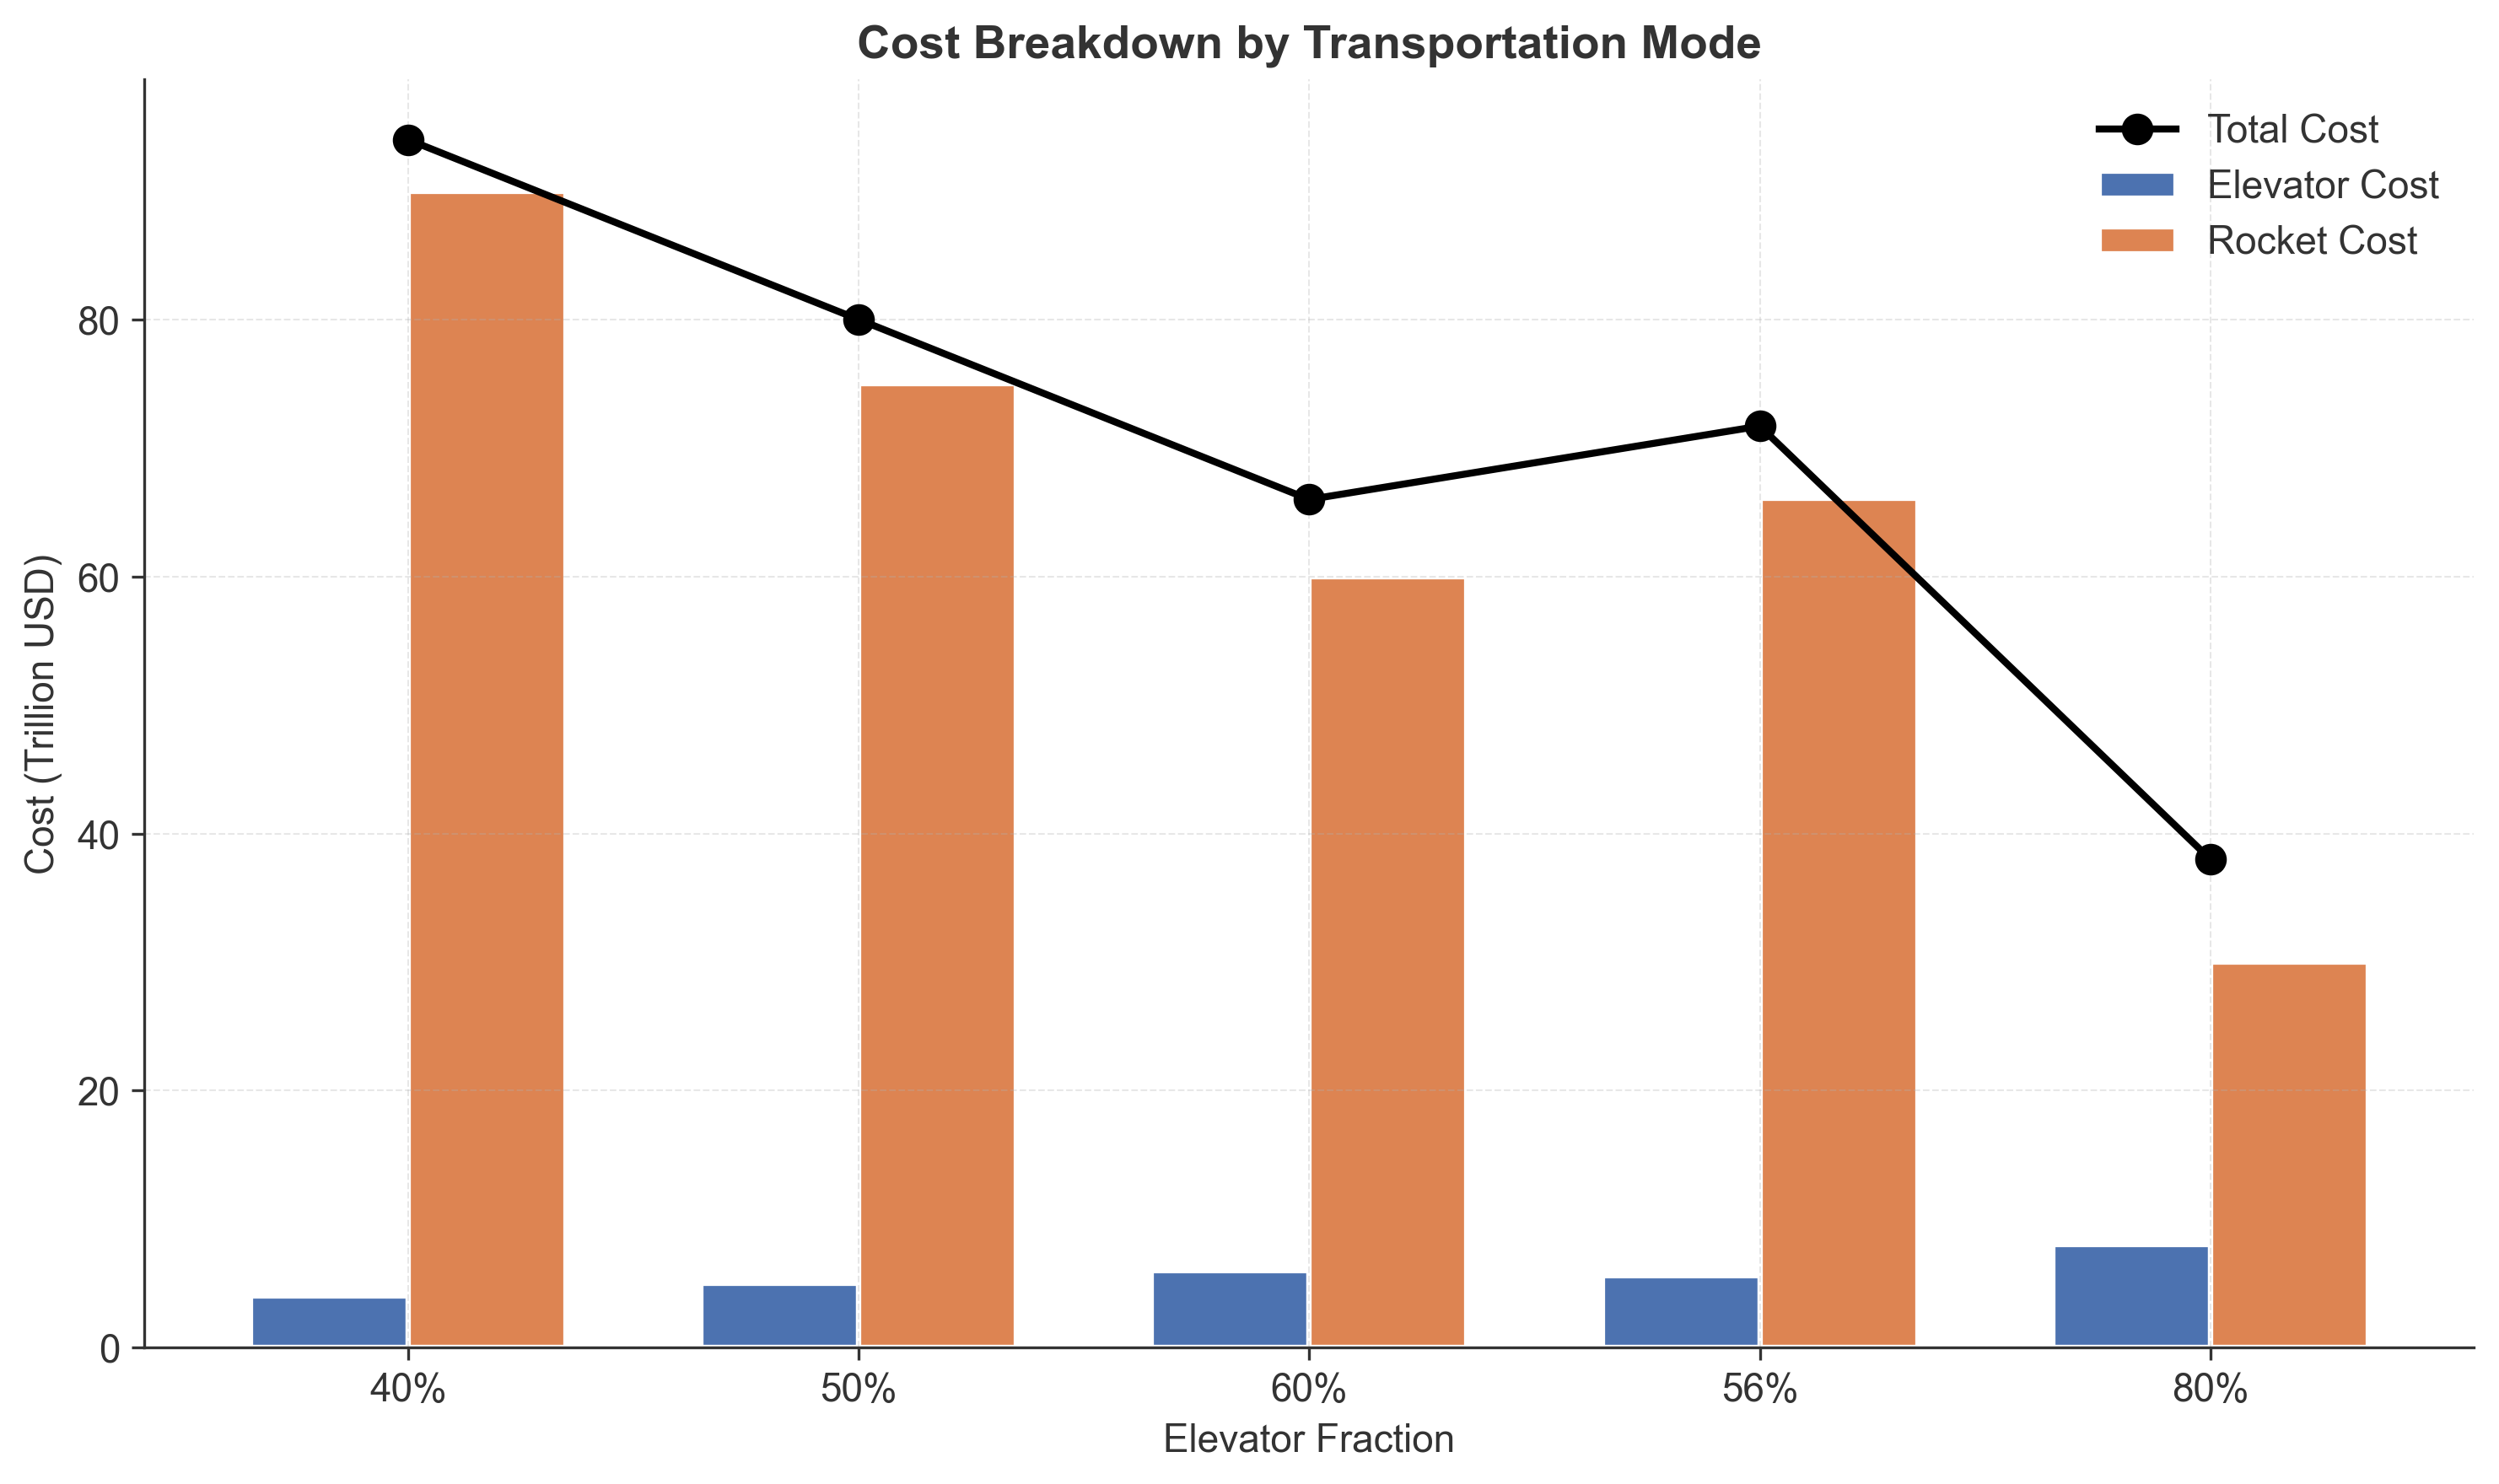
\includegraphics[width=0.95\textwidth]{../figures/fig_07_cost_breakdown.png}
    \caption{按运输模式分解的成本构成。随着电梯比例增加，电梯成本线性增长而火箭成本下降，黑色折线显示总成本变化趋势。}
    \label{fig:cost_breakdown}
\end{figure}

图~\ref{fig:cost_breakdown}详细展示了不同混合配置下的成本构成分解。

\subsubsection{模型三结果小结}

\begin{table}[htbp]
    \centering
    \caption{混合方案优化结果}
    \label{tab:hybrid_results}
    \begin{tabular}{lrr}
        \toprule
        指标 & 数值 & 单位 \\
        \midrule
        最优电梯比例 & 55.9 & \% \\
        电梯运输量 & 5592 & 万公吨 \\
        火箭运输量 & 4408 & 万公吨 \\
        合计年运力 & 894,010 & 公吨/年 \\
        建设周期 & 111.9 & 年 \\
        完工年份 & 2162 & -- \\
        总成本 & 71.71 & 万亿美元 \\
        电梯成本占比 & 5.59 & 万亿美元 \\
        火箭成本占比 & 66.12 & 万亿美元 \\
        总CO$_2$排放 & 181.9 & 百万公吨 \\
        \bottomrule
    \end{tabular}
\end{table}

混合方案相比纯电梯方案缩短工期\textbf{41.1\%}，相比纯火箭方案缩短\textbf{55.9\%}，成本处于两极端之间。

\subsection{模型四：系统可靠性与环境可持续性}

\subsubsection{非完美条件下的可靠性分析}

实际运输系统会经历故障、维护需求和运营中断，偏离理想假设。本模型检验不同故障率如何影响任务结果。

\paragraph{故障情景分析}

通过参数化故障率$\epsilon_e \in [0, 0.20]$（电梯）和$\epsilon_r \in [0, 0.20]$（火箭），对每种配置重新计算有效运力并预测工期影响。

\begin{figure}[htbp]
    \centering
    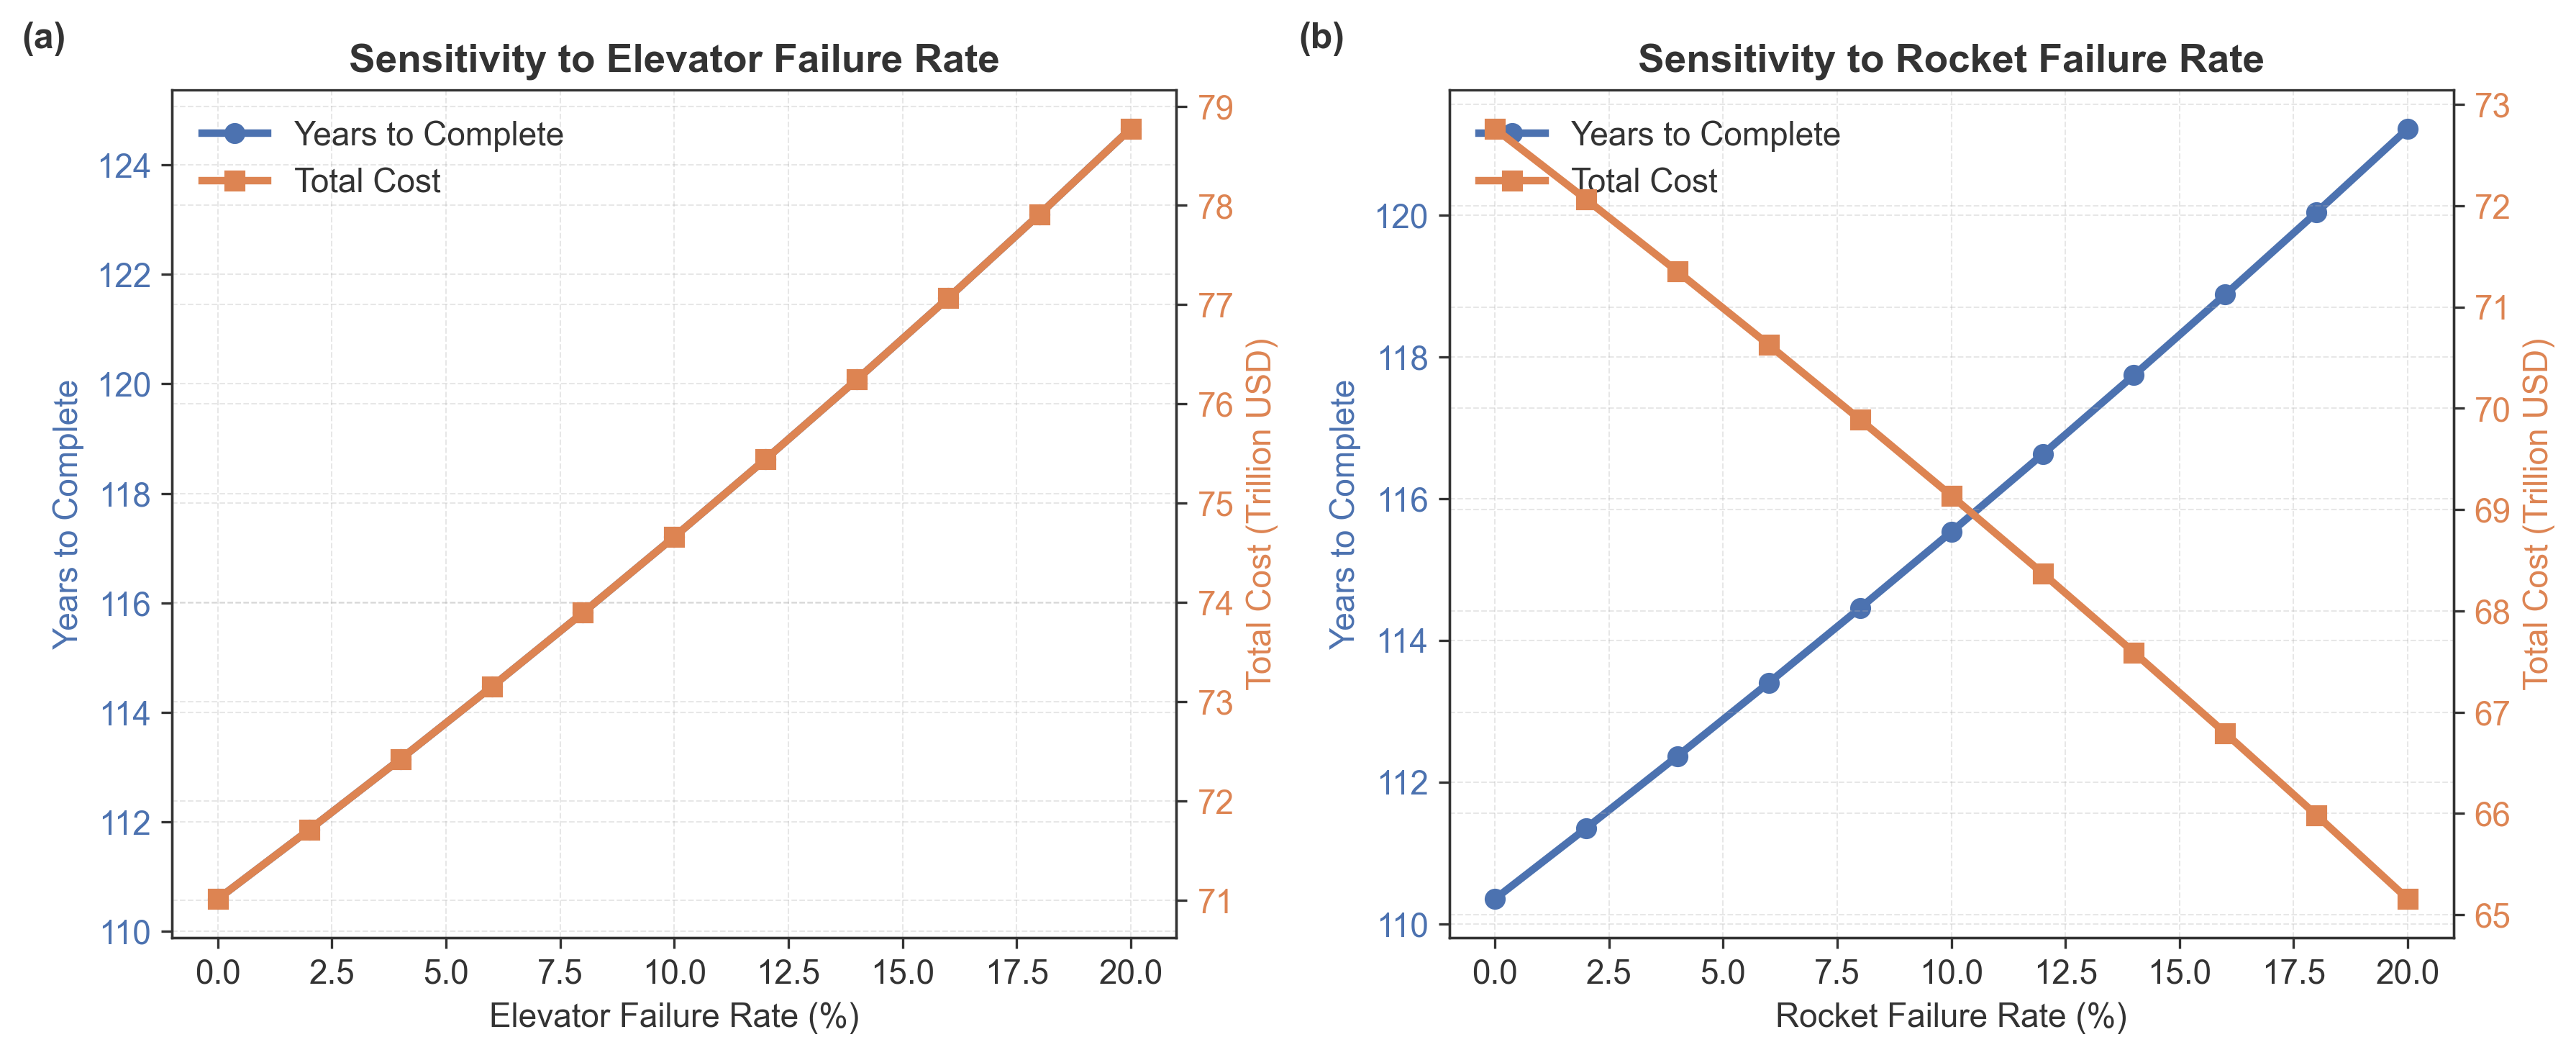
\includegraphics[width=0.95\textwidth]{../figures/fig_04_sensitivity_analysis.png}
    \caption{建设周期和成本对系统故障率的敏感性分析：(a)混合方案对电梯故障率的敏感性；(b)对火箭故障率的敏感性。故障率升高通过降低有效运力延长工期并增加成本。}
    \label{fig:sensitivity_analysis}
\end{figure}

如图~\ref{fig:sensitivity_analysis}所示，电梯故障率从2\%升至12\%使混合方案工期延长约\textbf{12.3\%}（从112年至126年）。同等幅度的火箭故障率增加仅导致\textbf{4.2\%}工期延长，因为火箭在最优混合配置中的运力贡献较小。

这种不对称性揭示了重要洞见：\textit{混合方案的性能对太空电梯可靠性比对火箭可靠性更敏感}，强调了健全的电梯维护协议的重要性。

\subsubsection{运营殖民地的水可持续性}

月球殖民地达到10万人规模后，持续运营需要不间断的供给运输。水是最关键的消耗品，对饮用、卫生、农业和工业过程不可或缺。

\paragraph{用水需求模型}

假设闭环循环系统实现90\%的水回收，人均日净水消耗估计为$W_{\text{daily}} = 15$升。殖民地年用水需求：
\begin{equation}
    W_{\text{annual}} = P \times W_{\text{daily}} \times 365 = 100,000 \times 15 \times 365 = 547,500,000 \text{ 升} = \textbf{547,500 公吨}
    \label{eq:water_requirement}
\end{equation}

\paragraph{供水运输成本比较}

\begin{figure}[htbp]
    \centering
    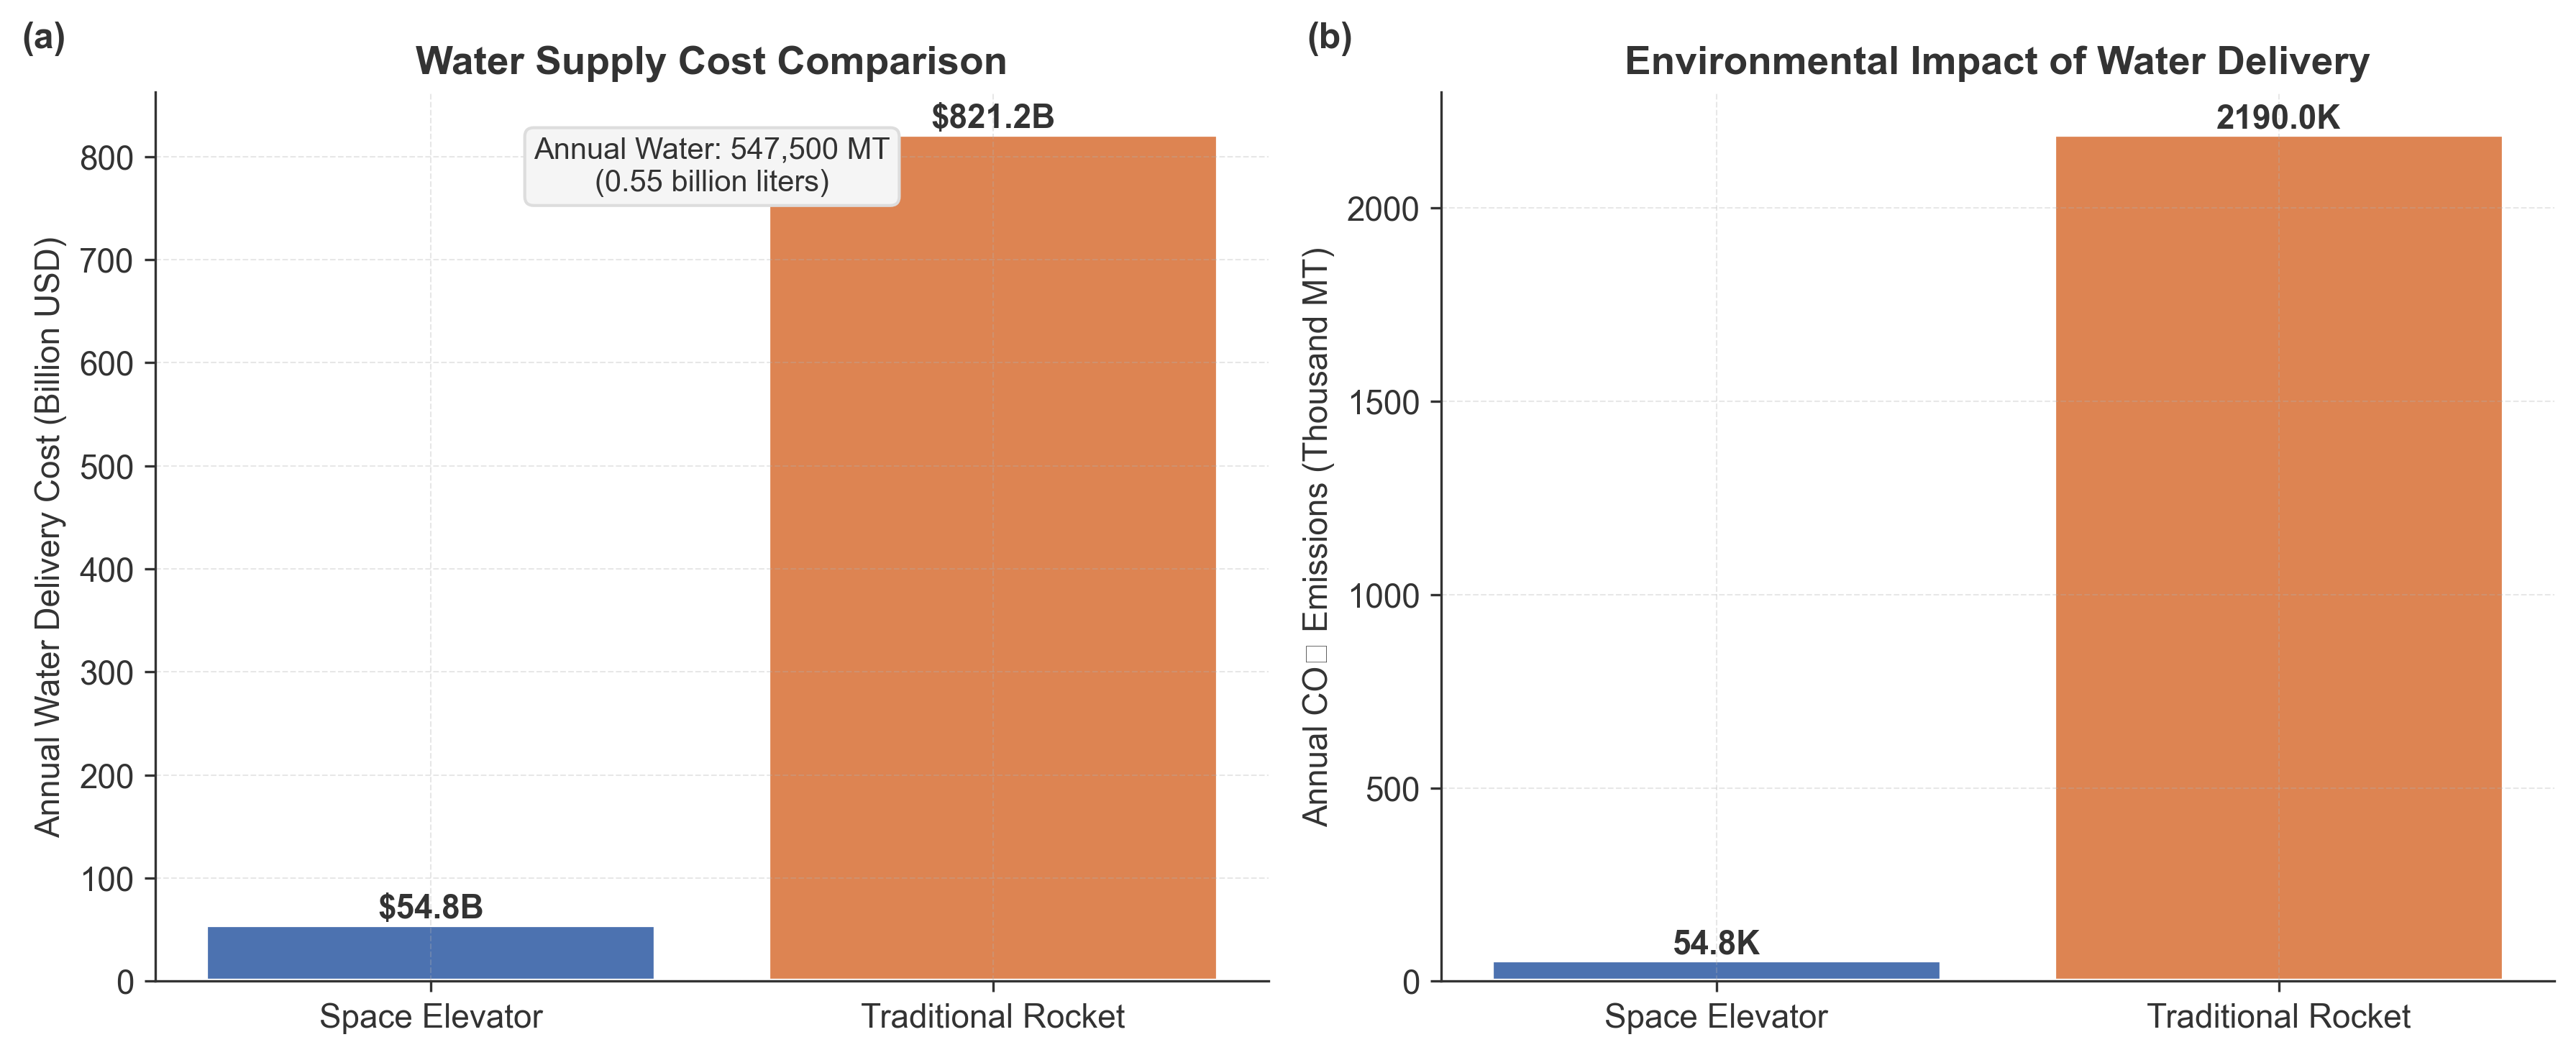
\includegraphics[width=0.95\textwidth]{../figures/fig_05_water_analysis.png}
    \caption{供水分析：(a)太空电梯与火箭运输的年度成本比较；(b)年度供水运输的环境影响。电梯运输具有\textbf{93.3\%}的成本优势。}
    \label{fig:water_analysis}
\end{figure}

图~\ref{fig:water_analysis}比较了供水运输成本：
\begin{align}
    \text{Cost}_{\text{water,elevator}} &= 547,500 \times 1000 \times 100 = \textbf{547.5 亿美元/年} \\
    \text{Cost}_{\text{water,rocket}} &= 547,500 \times 1000 \times 1,500 = \textbf{8212.5 亿美元/年}
\end{align}

太空电梯仅在供水运输方面就实现年节省\textbf{7665亿美元}，凸显其对殖民地长期可持续性的关键重要性。

\subsubsection{环境影响评估}

\begin{figure}[htbp]
    \centering
    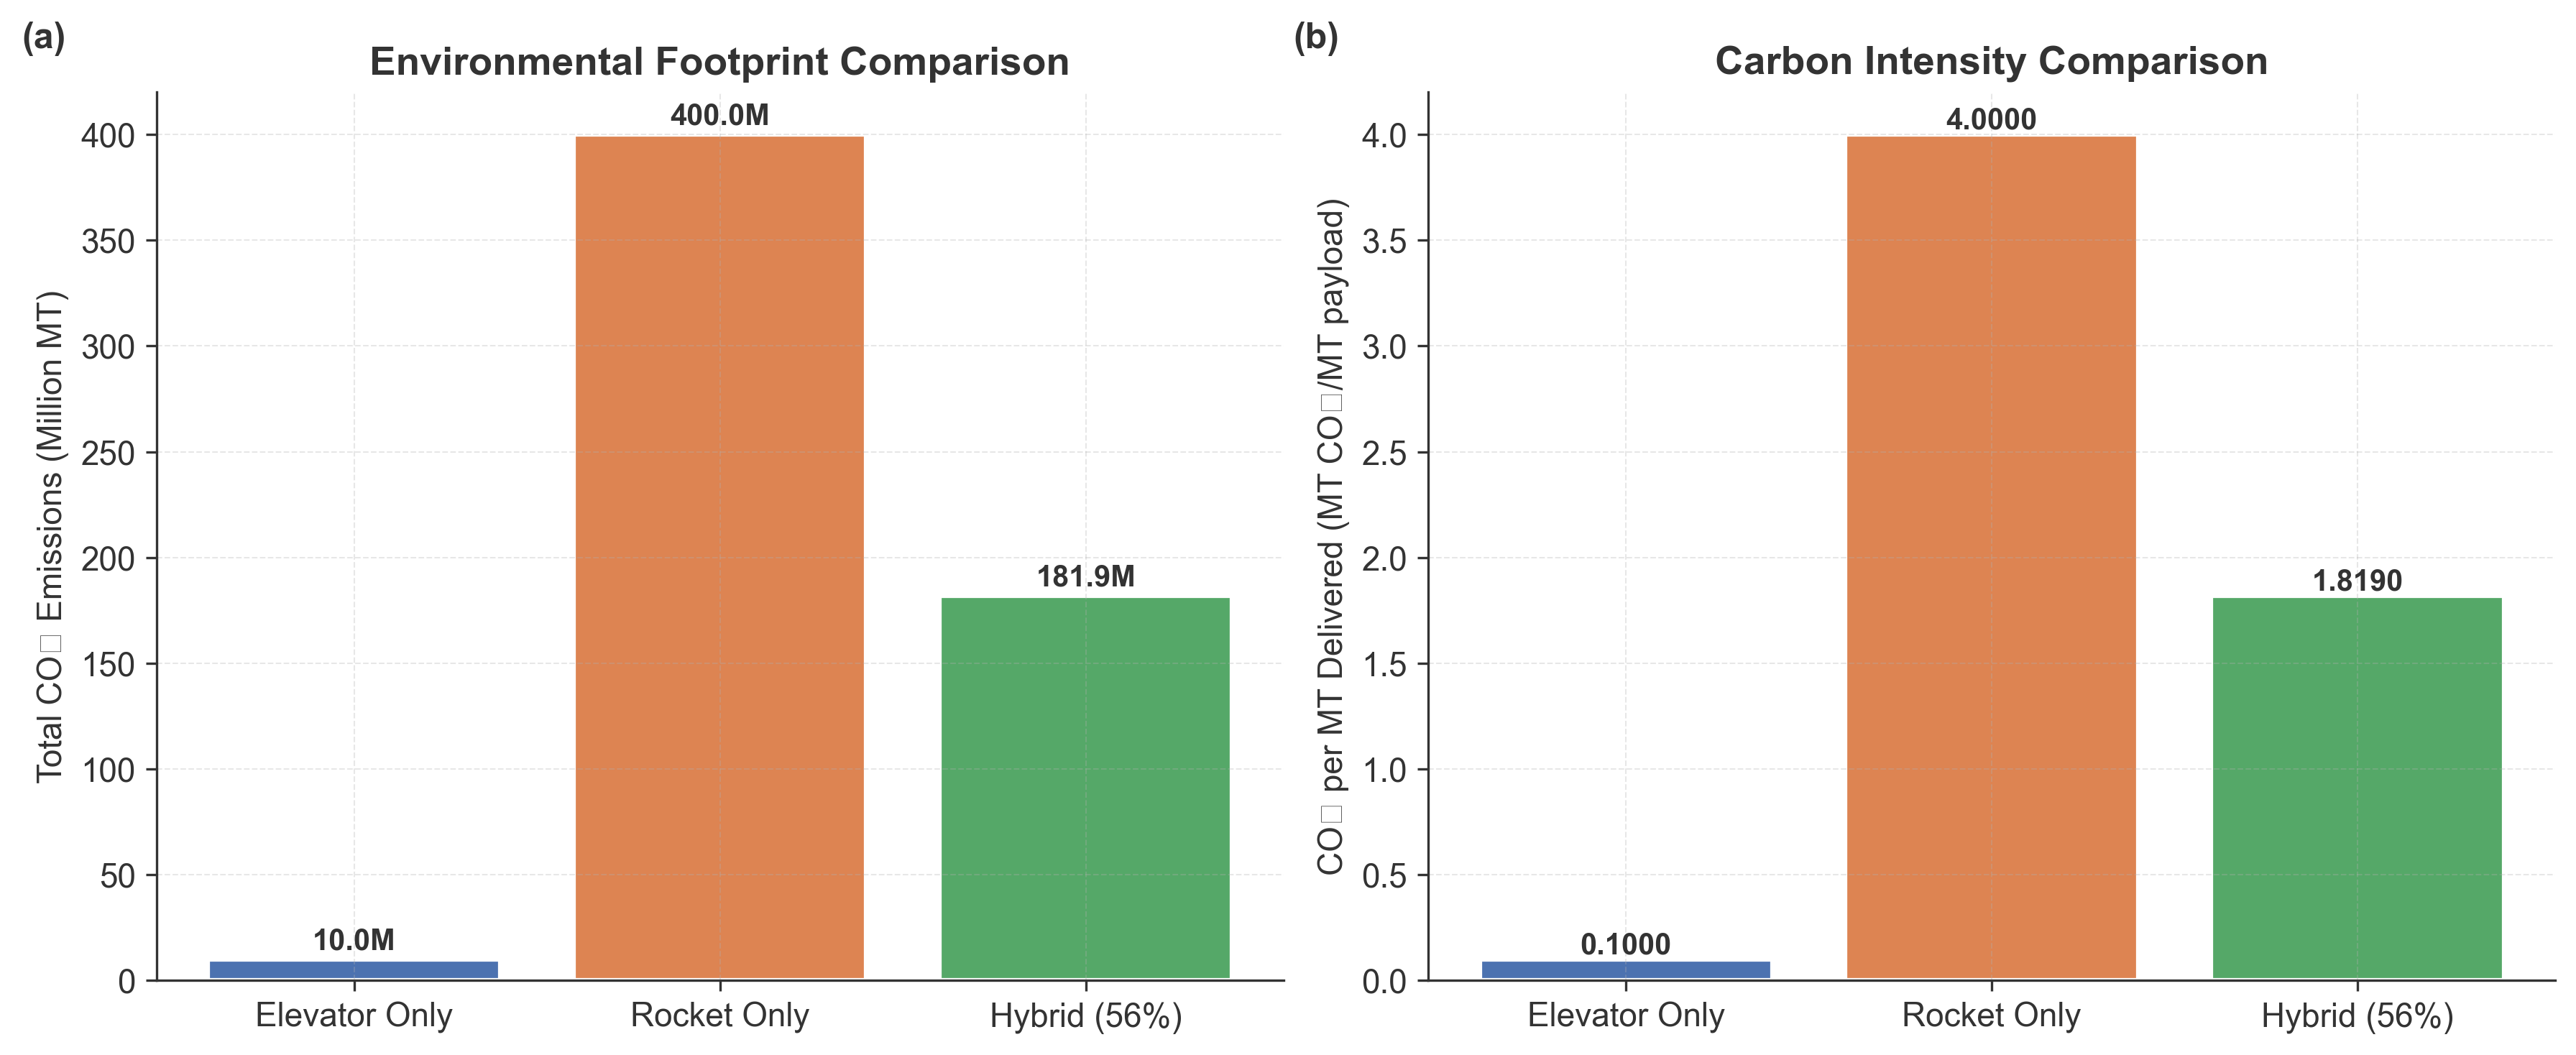
\includegraphics[width=0.95\textwidth]{../figures/fig_08_environmental_impact.png}
    \caption{环境足迹比较：(a)完整建设阶段的总CO$_2$排放；(b)单位载荷碳强度。太空电梯实现比火箭低\textbf{40倍}的碳强度。}
    \label{fig:environmental_impact}
\end{figure}

图~\ref{fig:environmental_impact}量化了环境差异：
\begin{enumerate}
    \item 电梯碳强度：\textbf{0.10}公吨CO$_2$/公吨载荷
    \item 火箭碳强度：\textbf{4.00}公吨CO$_2$/公吨载荷
\end{enumerate}

混合方案（1.819亿公吨CO$_2$）相比纯火箭方案（4亿公吨）减排\textbf{54.5\%}，而纯电梯方案实现\textbf{97.5\%}减排。

\paragraph{环境优化建议}

为在满足工期约束的同时最小化环境影响，建议：
\begin{enumerate}
    \item \textbf{最大化电梯利用}：优先使用电梯运输所有非时间紧迫材料。
    \item \textbf{绿色火箭燃料}：过渡到产生水蒸气而非CO$_2$的氢氧推进系统。
    \item \textbf{碳抵消计划}：投资相当于任务排放量的陆地碳捕获。
    \item \textbf{月球资源利用}：开发原位资源开采以逐步减少地球基材料需求。
\end{enumerate}
